\section{Implementation}\label{sect:realization}

This section illustrates how to practically implement \shortname. 
\newline
As we anticipated in Sections~\ref{sect:introduction} and~\ref{sect:background}, the following two technologies are the pillars of our construction:
\begin{itemize}
	\item the blockchain, the technological layer which allows us to publicly store the evolution of each instance of \shortname and persistently disclose the secret associated to it;
	\item smart contracts, the framework that permits to trigger economic incentives and penalties in a fully decentralized way, thus avoiding the need of trusted parties.
	%\item secure Multy-Party Computation, the instrument through which it is possible to securely execute bulletproof cryptographic operations between multiple hosts.
\end{itemize}
The combination of the the two with the model described in Section~\ref{sect:model}, constitutes \shortname: a generic protocol to deploy instances of the TL abstraction.
% without the need of trusted third parties or cryptographic puzzles.
Several realizations of the \shortname protocol can be obtain by changing the implementation of the \texttt{generate\_shares} primitive and the cryptographic techniques (e.g., oblivious transfer, probabilistic encryption, and sMPC) used to provide the shares only to the legitimate shareholder, while sending the commitments to the owner.
In this chapter we implement the \texttt{generate\_shares} primitive leveraging secure Multi-Party Computation.
%, therefore we discuss the implementation details of $\shortnamempc$.
In particular, we employ a modular arithmetic sMPC to be able to compute the shares using Shamir's Secret Sharing.
In addition, we use the {\em \mimc}~\cite{albrecht2016mimc} algorithm to implement the \texttt{hash} primitive used to compute the commitments.
\mimc is a minimal multiplicative complexity hashing primitive that has the advantage of being composed of only modular arithmetic operations, and is thus suitable to be used in our arithmetic sMPC
%The advantage of its use is twofold: low gas price spent in contract calls, and lower sMPC execution time
(further details on this in Section~\ref{sect:evaluation}).
  

%A brief description of the some of the technical issues, which have to be solved to get a correct execution, is now given. 
%Moreover, it emerges the need to manage the coordination among all the participants. 
%In fact, before being able to proceed with some actions, \shortname stands in need of consensus among all the participants, and not only among the majority of them. 
%As an example the owner might desire all the shareholders to deposit their bids before distributing the shares.

\begin{figure*}[t]
	\centering
	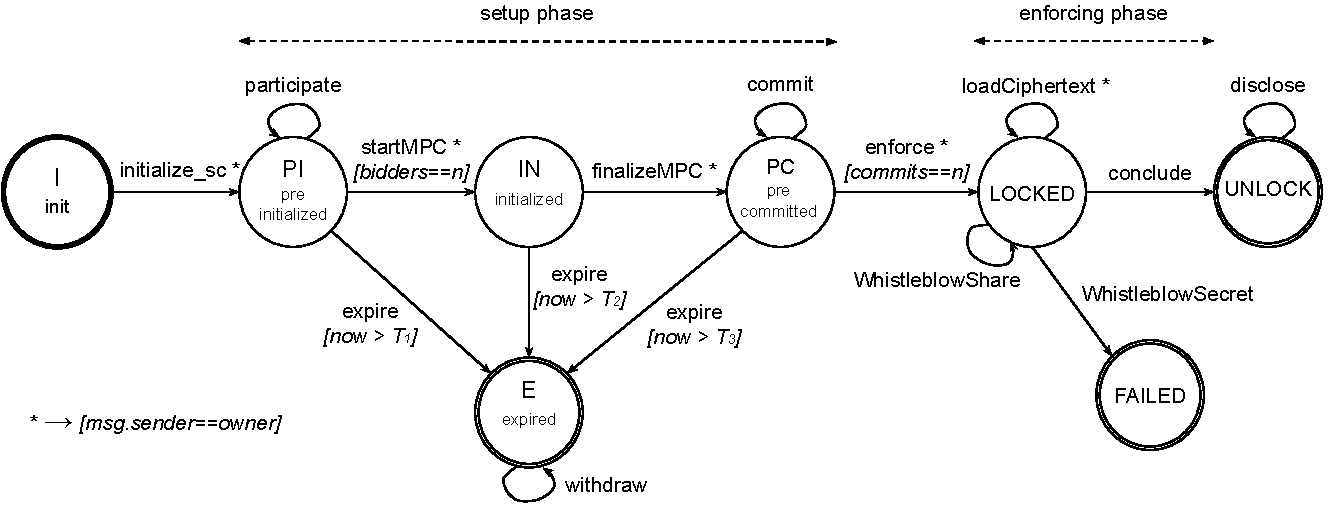
\includegraphics[width=0.9\textwidth]{fig/protocol_fsm_simple_version.pdf}
	\caption{State machine representing the valid transitions of the $\shortnamempc$ protocol. Each transition name maps to an action (an Ethereum smart contract function) that can be invoked by each participant in order to modify the state. Square brackets contain additional conditions to be met to make valid transitions}
	\label{fig:fsm}
\end{figure*}

\subsection{The \shortname state machine}\label{sect:ityt_exec}
 
We designed $\shortnamempc$ as a finite state machine implemented in an Ethereum smart contract.
The state of each of its instances can be evolved by performing actions that map to specific smart contract functions.
Before performing any update, each function first verifies that the state machine is in the expected state, and terminates otherwise.
A simplified version of the state machine that only shows valid transitions is presented in Figure~\ref{fig:fsm}.
The state machine is characterized by three main phases: the \texttt{setup} phase, in which the owner has to deploy the contract and the shareholders have to commit to take part to it; the \texttt{activation} phase, in which the shareholders declare that they received their shares and give their go-ahead; and the \texttt{enforcing} phase, in which the participants comply with the constraints of the contract thus effectively realizing the TL primitive as a consequence.
%
%Furthermore, before participating to a specific instance, each candidate can verify the algorithmic code contained inside the contract. 
%
%The \texttt{setup} phase involves {\em off-chain} operations (i.e., not directly performed by the smart contract functions), therefore it can also be divided in two steps: {\em deployment} and {\em activation}.
In between the \texttt{setup} and the \texttt{activation} phases, the owner and the shareholders collaboratively execute the {\em off-chain} sMPC protocol that generates and distributes the shares and the commitments.
These phases are discussed in details in the following.

\medskip

\paragraph*{Setup phase}
Initially, the owner deploys a smart contract instance of $\shortnamempc$ on the Ethereum blockchain.
As detailed in Algorithm~\ref{algo:init}, the owner invokes the \texttt{initialize\textunderscore sc} primitive, she transfers \PO to the contract and she specifies all the instance parameters detailed in Section~\ref{sect:model}.
%able to specify: (i) the shareholder identifiers, (ii) the economic parameters, and (iii) the time threshold required for the desired execution.
This advances the protocol to the \texttt{PRE\_INITIALIZED} state. 
To demonstrate the will to correctly participate, each shareholder invokes the smart contract function \texttt{participate}, as part of Algorithm~\ref{algo:shareholder_commitment} and transfers to the contract the proper amount of Ether corresponding to the bid, $B_{\mathcal{H}}$. 
The owner observes the actions taken by all the participants by reading the state of the contract and, after she ensured that all the shareholders have deposited their bids, she invokes the function \texttt{startMPC} which permits to advance the state to \texttt{INITIALIZED}.
This opens the off-chain sMPC window, in which all the participants cooperate to realize the \texttt{generate\_shares} protocol.

\medskip

\paragraph*{Off-chain sMPC}\label{sect:impl_mpc_brief}
The sMPC permits to generate the shares of the secret, confidentially distribute them to the shareholders, while forwarding the commitments to the owner.
However, it is executed when the TL instance is still inactive, or rather when the economic penalties have not been activated yet. 
To avoid the exposition of \secret, the owner introduces a fictitious random key, \key.
The key is submitted to the sMPC instead of the secret, and a set of $n$ shares $\left\lbrace \share _1 , \ldots , \share_{n} 	\right\rbrace$, is produced.
Specifically, the shares are derived from the key using the Shamir's Secret Sharing algorithm~\cite{Shamir:1979:SS:359168.359176}, so that it is possible to reconsruct $\key$ out of \KofN shares.
Accordingly, the owner can wait to the activation of the TL, and then upload into the smart contract the encrypted version (i.e., the ciphertext) of the secret, $\ciphertext = $ \wrapsecret. 
%The scenario is illustrated in 
Figure~\ref{fig:key_delayed_wrap} illustrates the scenario.

To execute the sMPC protocol the owner has to input the random key, \key, together with the total number of shareholders, $n$, and the reconstruction threshold, $k$. 
Each shareholder, instead, submits only a random seed.
The sMPC generates internally random values which are interpreted as the $x$ coordinates by the Shamir's Secret Sharing algorithm.
Each $i$-th share is then generated by the concatenation of $x_i$ and $y_i$ coordinates.
As output of the sMPC protocol, $\owner$ receives a commitment $\commitment _i$ of any share generated~\footnote{By share commitment we denote the MiMC hash of the share.}, while each shareholder receives her share $\share_{i}$, a commitment of the key $ \commitment _ \key $, $n$ and $k$.
A graphical view of the discussed sMPC protocol is shown in Figure~\ref{fig:mpc1}.
%Other useful implications will be explained in the \texttt{enforcing} phase. 

We remark that the sMPC permits to keep the input and output of each participant private, thus ensuring to each shareholder that no one, except herself, will be able to submit her share at disclosure time. 
This is pivotal to guarantee the economic game conditions over which our analysis is based. 
%Further important implications about the use of an sMPC will be discussed later, in Subsection~\ref{sect:impl_mpc}.

\medskip

\paragraph*{Activation phase}
When the sMPC terminates the owner invokes the function \texttt{finalizeMPC} and updates the smart contract state with the commitment of the key, $ \commitment _\key $, along with the commitments of all the shares, $\{ \commitment _1 , ... , \commitment _n \}$. 
As a consequence, the state of \shortname turns to \texttt{PRE\_COMMITTED}. 
Each shareholder is now asked to verify the correctness of the data deposited in the contract by $\owner$. 
In particular, if the commitment written by the owner matches to the one given by the shareholder (i.e., the owner did not tamper $\commitment_i$), then each shareholder would invoke the \texttt{commit} function. 
After each of them committed, the owner invokes \texttt{enforce}, which activates the TL (i.e., activation of all economic incentives and penalties). 
The state turns to \texttt{LOCKED}, and the \texttt{activation} phase ends.

The \texttt{setup}, \texttt{off-chain sMPC}, and \texttt{activation} phase together realize the Algorithms~\ref{algo:init} and~\ref{algo:shareholder_commitment}, needed to conclude the setup of the \shortname instance. 

\medskip

\paragraph*{Enforcing phase}\label{sect:impl_enf_brief}

Before disclosure time, the smart contract permits to: (i) whistleblow a single share, and (ii) whistleblow the secret.
If the commitment matches the value stored in the contract, then $\Wbonus_{\share}$ is immediately paid to the whistleblower.
A share whistleblow is permitted only $\K - 1 $ times, as a greater number of submission leads the TL to the \texttt{FAILED} state.
When that happens the remaining amount locked by the contract is destroyed.
%Contrary to the previous case, the possession of \key demonstrates either its mismanagement by the owner or the collusion among the shareholders, and in this setting it is impossible to discriminate between them.   

If no adversarial coalition reconstructs \key before the disclosure time \td, then all the shareholders will be able to disclose their shares by invoking the function \texttt{disclose} (Algorithm~\ref{algo:disclose}).
Each share is considered valid only if it matches the corresponding commitment.
In that case, a reward will be paid to the shareholder conditionally to the outcome of the instance (i.e., the TL ends successfully only if at least $\K$ valid shares are submitted before $\te$).
There is no need to materialize \key or \secret in the smart contract, as all the valid shares will be permanently and publicly accessible. Anyone can recover \key from the shares and then extract the plaintext performing the decryption operation, \secret $=$ \unwrap.

\begin{figure}[t]
	\centering
	\subfloat[A colluding coalition could reveal \secret before contract activation] {{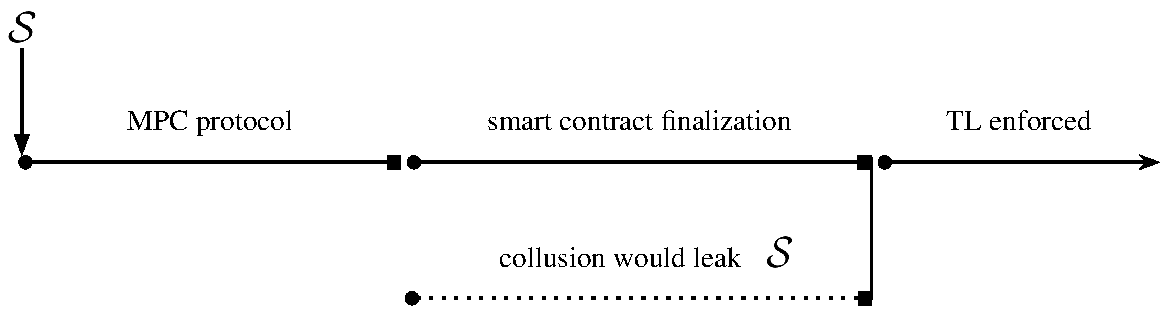
\includegraphics[width=0.9\columnwidth]{fig/time1} }}\\
	\vspace*{2pt}
	\subfloat[A colluding coalition could only reveal \key before contract activation] {{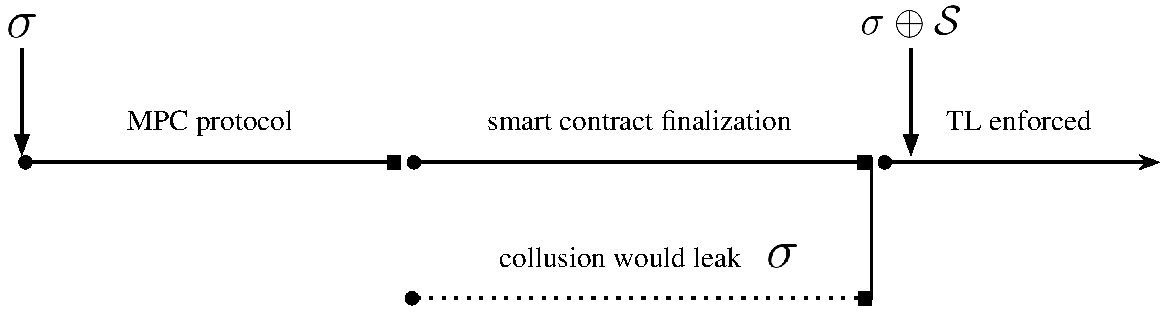
\includegraphics[width=0.9\columnwidth]{fig/time2} }}
	\caption{Preventing secret exposure before smart contract activation}%
	\label{fig:key_delayed_wrap}%
\end{figure}


Up until now, the protocol has only been based on the key \key, but the \secret has not been offloaded to the TL yet.
%Indeed, uploading \ciphertext into the smart contract is (counter-intuitively) optional, as the implementation is totally agnostic to the presence of \ciphertext or to the meaning of \secret. 
The explanation is straightforward: the outcome of $\shortnamempc$ is only bounded to the disclosure of the key, to which all the incentive and penalties are related to. 
As soon as the state of the TL advances to \texttt{LOCKED} and before going offline, the owner encrypts the secret \secret as shown in Section~\ref{sect:impl_mpc_brief} in order to obtain the \ciphertext. Then she invokes the smart contract function \texttt{loadSecret} to store the \ciphertext in the smart contract.